\section{1184003 - Dinda Anik Masruro}
\subsection{Teori}
\begin{enumerate}

	\item Jelaskan apa itu binary classification dilengkapi ilustrasi gambar sendiri.
	\hfill\break
    Binary Classification merupakan sebuah metode untuk menklasifikasikan elemen yang dibentuk seperti grup dan nantinya akan  dibagi menjadi 2 grup. Dari 2 grup tersebut diprediksikan setiap anggota pada grup yang mana sesuai dengan yang diatur pada aturan klasifikasi. Data atau konteks yang didapat membutuhkan keputusan dari item tersebut memiliki properti kualitatif, karakteristik yang spesifik, atau tipikal klasifikasi biner.

	\begin{figure}[h]
	\centering
		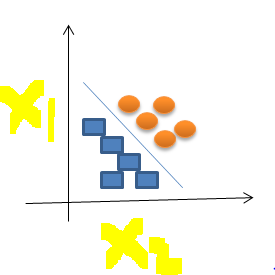
\includegraphics[width=4cm]{figures/1184003/chapter2/1.PNG}
		\caption{Binary classification.}
	\end{figure}

	\item Jelaskan apa itu supervised learning dan unsupervised learning dan clustering dengan ilustrasi gambar sendiri.
	\hfill\break

	\begin{itemize}
		\item Supervised Learning
		\hfill\break Supervised Learning	merupakan algoritma yang memiliki attribut tambahan seperti x dan y yang ingin diprediksi.
		
		\begin{figure}[h]
		\centering
			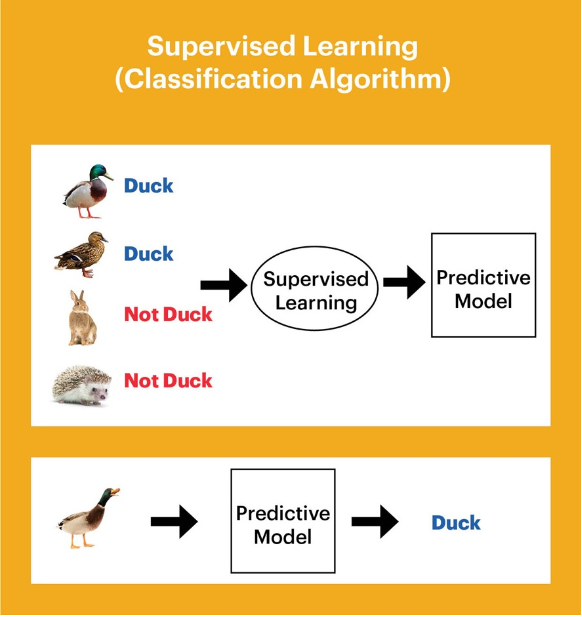
\includegraphics[width=3cm]{figures/1184003/chapter2/2.PNG}
			\caption{Supervised Learning.}
		\end{figure}
		\newpage\item Unsupervised Learning 
		\hfill\break
		Unsupervised Learning  merupakan	algoritma yang tidak memiliki attribut tambahan yang akan diprediksi.
		\begin{figure}[h]
		\centering
			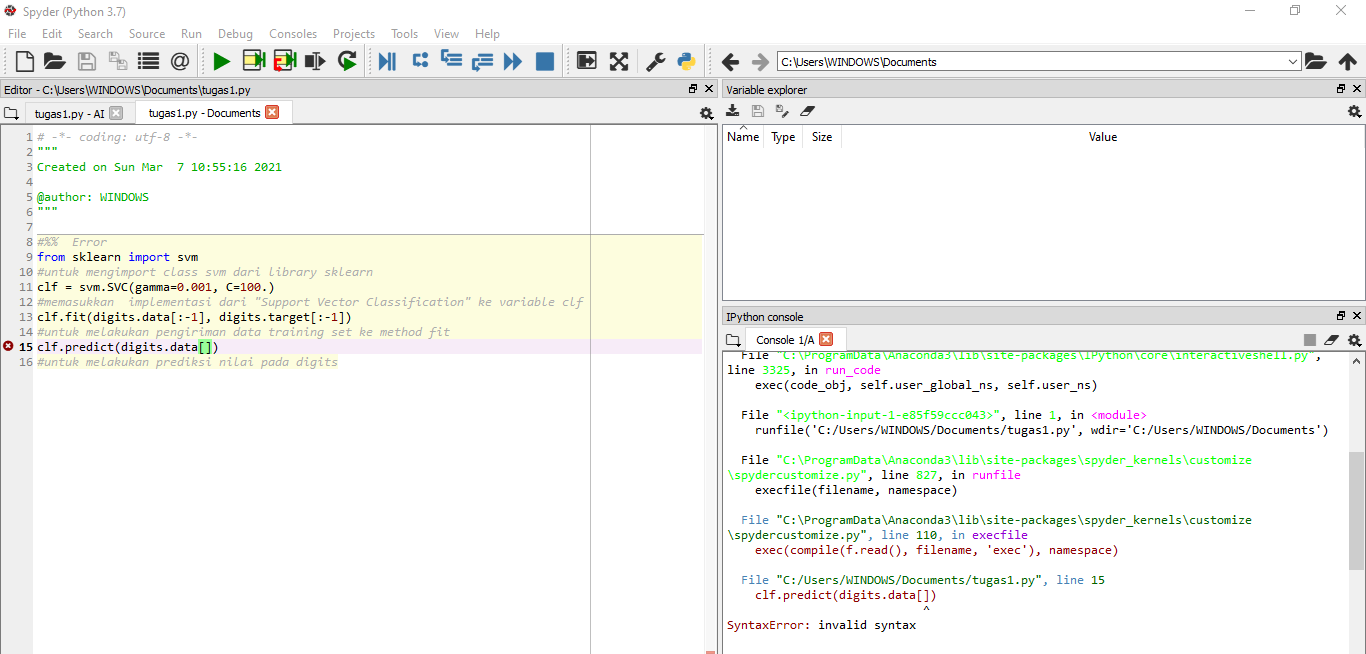
\includegraphics[width=3cm]{figures/1184003/chapter2/3.PNG}
			\caption{Unsupervised Learning.}
		\end{figure}

		\item Clustering
		\hfill\break
		Clustering adalah peroses mengklasifikasikan yang berdasarkan suatu parameter dalam penentuannya contoh pada berat buah, buah A memiliki berat 100 gr dan buah B memiliki berat 120 gr yang berarti berat buah dibagi dua parameter yaitu lebih kecil samadengan 100 gram dan lebih besar dari gram contoh pada gambar.
		\begin{figure}[h]
		\centering
			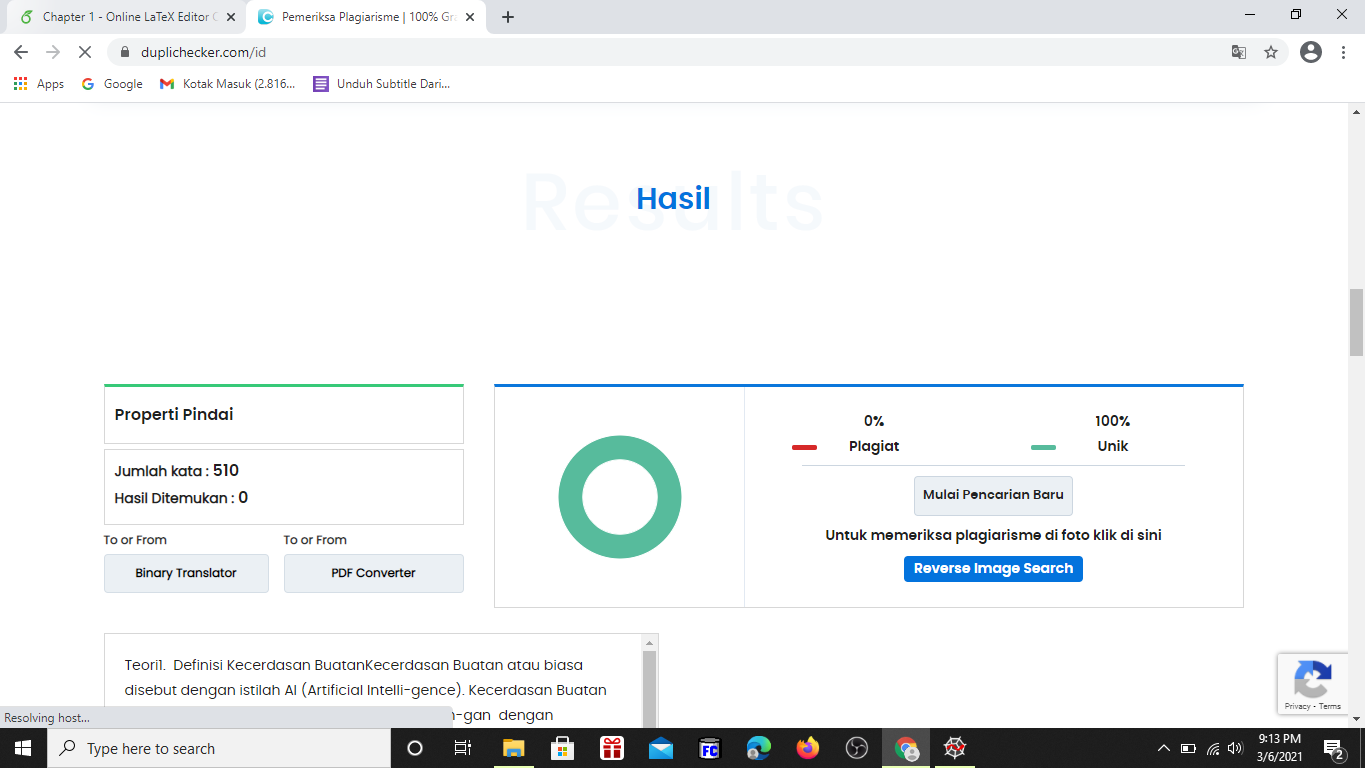
\includegraphics[width=3cm]{figures/1184003/chapter2/4.PNG}
			\caption{Clustering.}
		\end{figure}
	\end{itemize}
	
	\item Jelaskan apa itu evaluasi dan akurasi dari buku dan disertai ilustrasi contoh dengan gambar sendiri.
	\hfill\break
	Evaluasi adalah tentang bagaimana kita dapat mengevaluasi seberapa baik model bekerja dengan mengukur tingkat akurasinya.Sedangkan akurasi akan didefinisikan sebagai persentase kasus yang diklasifikasikan dengan benar. Kita dapat menganalisis kesalahan yang dibuat oleh model,atau tingkat kebingungannya, menggunakan matriks kebingungan(confusion matrix). Matriks kebingungan mengacu pada kebingungan dalam model,tetapi matriks kebingungan ini bisa menjadi sedikit sulit untuk dipahami ketika mereka menjadi sangat besar.
	\begin{figure}[h]
	\centering
		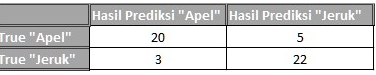
\includegraphics[width=10cm]{figures/1184003/chapter2/5.PNG}
		\caption{Evaluasi dan Akurasi.}
	\end{figure}

	\item Jelaskan bagaimana cara membuat dan membaca confusion matrix, buat confusion matrix buatan sendiri.
	\hfill\break
	\begin{enumerate}
	\item Cara membuat dan membaca confusion matrix :
	\begin{itemize}
	\item Confusion Matrix merupakan metode untuk menghitung akurasi pada data mining atau Sistem Pendukung Keputusan. Untuk menggunakan Confusion Matrix, ada 4 istilah sebagai hasil proses dari klasifikasi. Diantaranya adalah:
	\item True Positive: Data positif yang terdeteksi memiliki hasil benar
    \item False Positive: Data Positif yang terdeteksi memiliki hasil salah
    \item True Negative: Data negatif yang terdeteksi memiliki hasil benar
    \item False Negative: Data negatif yang terdeteksi memiliki hasil salah
	\end{itemize}
	\end{enumerate}
	\begin{figure}[h]
	\centering
		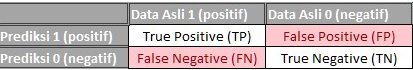
\includegraphics[width=7cm]{figures/1184003/chapter2/6.PNG}
		\caption{Confusion Matrix.}
	\end{figure}

	\item Jelaskan bagaimana K-fold cross validation bekerja dengan gambar ilustrasi contoh buatan sendiri.
	\hfill\break
	K-fold cross validation adalah salah satu metode untuk mendapatkan kinerja classifier, 
	metode ini dapat digunakan dengan jumlah data yang terbatas (tidak banyak contoh).
	Cara kerja K-fold cross validation adalah sebagai berikut
	\begin{itemize}
	\item Total instance dibagi menjadi N bagian.
		\item Fold-1 adalah ketika bagian 1 menjadi data uji (data pengujian) dan sisanya menjadi data pelatihan (data pelatihan).
		\hfill\break
		Selanjutnya, hitung keakuratan berdasarkan porsi data. Perhitungan akurasi menggunakan persamaan berikut:
		Akurasi = sigma data uji benar klasifikasi sigma total data uji x 100%%
		\item Fold ke-2 adalah ketika bagian ke-2 menjadi data uji (data pengujian) dan sisanya menjadi data pelatihan (data pelatihan).
		\hfill\break
		Selanjutnya, hitung keakuratan berdasarkan porsi data.4. 
		Demikian seterusnya hingga mencapai fold ke-K. 
		Hitung rata-rata akurasi dari K buah akurasi di atas. 
		Rata-rata akurasi ini menjadi akurasi final.
	\end{itemize}

	\begin{figure}[h]
	\centering
		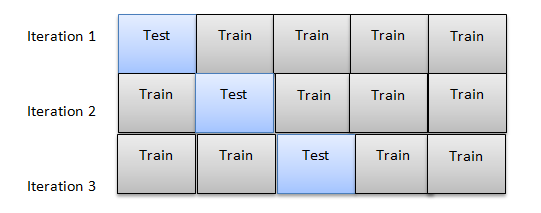
\includegraphics[width=5cm]{figures/1184003/chapter2/7.PNG}
		\caption{K-fold Cross Validation.}
	\end{figure}

	\item Jelaskan apa itu decision tree dengan gambar ilustrasi contoh buatan sendiri.
	\hfill\break
	Decision tree merupakan implementasi dari binari clasification dimana pada pohon keputusan akan terdapat root atau akar dan cabang cabangnya yang nilainya seperti if contoh pada root berisi nilai warna mawar, apakah merah pada cabang satu bernilai iya dan pada cabang dua bernilai tidak jika nilainya iya berarti mawar dan jika tidak maka bukan mawar.
    agar lebih jelas dapat dilihat pada gambar decision tree berikut:

	\begin{figure}[h]
	\centering
		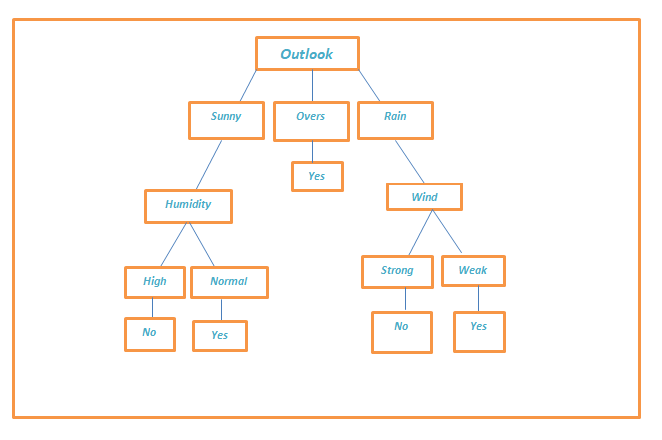
\includegraphics[width=4cm]{figures/1184003/chapter2/8.PNG}
		\caption{Decision Tree.}
	\end{figure}

	\item Jelaskan apa itu information gain dan entropi dengan gambar ilustrasi buatan sendiri.
	\hfill\break
	informasion gain merupakan informasi atau keriteria dalam pembagian sebuah objek contoh information gain pada ikan yaitu hidup di air, berkoloni, berinsang. untuk lebih jelasnya dapat dilihat pada gambar berikut :
	\begin{figure}[h]
	\centering
		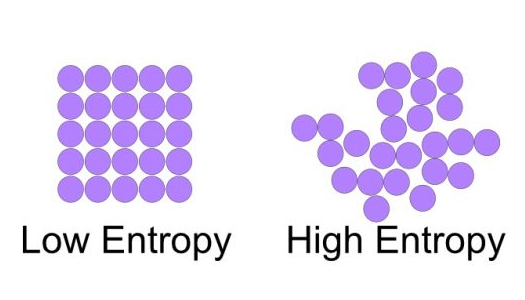
\includegraphics[width=6cm]{figures/1184003/chapter2/9.PNG}
		\caption{Entropi.}
	\end{figure}


\end{enumerate}


\subsection{Praktek}
\begin{enumerate}
	\item Soal 1
	\hfill\break
	\lstinputlisting[firstline=8, lastline=19]{src/1184003/chapter2/1184003.py}
	Kode di atas digunakan untuk mengimpor atau mengirim library pandas sebagai pd. Kemudian ditentukan variabel "anggur" untuk dipanggil dataset diperoleh dari data student-mat.csv. 
	\begin{figure}[h]
	\centering
		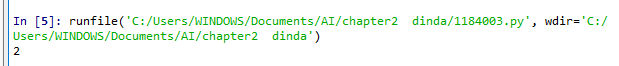
\includegraphics[width=4cm]{figures/1184003/chapter2/10.PNG}
		\caption{Hasil Soal 1.}
	\end{figure}
	\item Soal 2
	\hfill\break
	\lstinputlisting[firstline=20, lastline=28]{src/1184003/chapter2/1184003.py}
	Kode di atas ada bagian mendeklarasikan pass/fail nya data berdasarkan G1+G2+G3. Dengan ketentuan nilai pass nya yaitu sama dengan 30. kemudian pada variabel medan dideklarasikan jika baris dengan G1+G2+G3 ditambahkan, dan hasilnya sama dengan 35 maka axisnya 1.
	\begin{figure}[h]
	\centering
		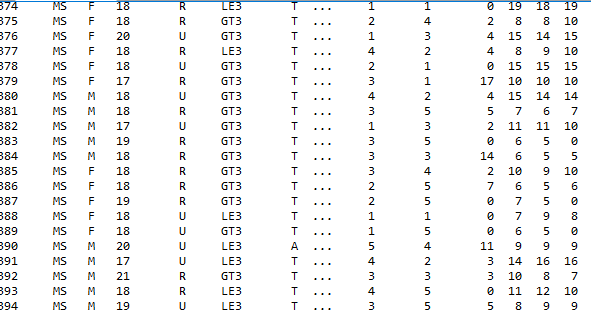
\includegraphics[width=3cm]{figures/1184003/chapter2/11.PNG}
		\caption{Hasil Soal 2.}
	\end{figure}
	\item Soal 3
	\hfill\break
	\lstinputlisting[firstline=29, lastline=34]{src/1184003/chapter2/1184003.py}
	One-hot encoding adalah proses di mana variabel kategorikal dikonversi menjadi bentuk yang dapat disediakan untuk algoritma ML untuk melakukan pekerjaan yang lebih baik dalam prediksi. Metode head ini digunakan untuk mengembalikan baris n atas 5 secara default dari frame atau seri data Karena saya memuat data menggunakan. 
	\begin{figure}[h]
	\centering
		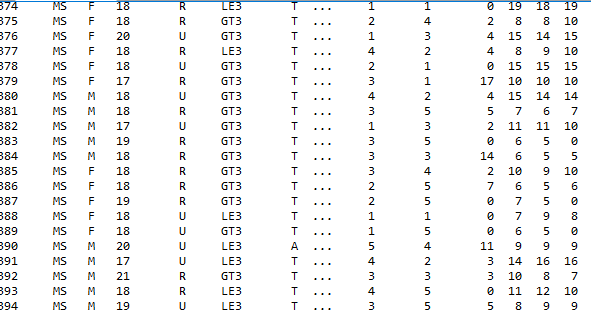
\includegraphics[width=3cm]{figures/1184003/chapter2/12.PNG}
		\caption{Hasil Soal 3.}
	\end{figure}
	\item Soal 4
	\hfill\break
	\lstinputlisting[firstline=35, lastline=59]{src/1184003/chapter2/1184003.py}
	Sample digunakan untuk mengembalikan sampel acak item dari objek. Pada bagian tersebut, terdapat train dan test yaing digunakan untuk untuk membagi train, test dan kemudian membagi lagi train ke validasi dan test. Kemudia akan mengimport module numpy sebagai np yang akan digunakan untuk mengembalikan nilai passing dari pelajar dari keseluruhan dataset dengan cara print.
	\begin{figure}[h]
	\centering
		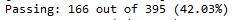
\includegraphics[width=3cm]{figures/1184003/chapter2/13.PNG}
		\caption{Hasil Soal 4.}
	\end{figure}
	\item Soal 5
	\hfill\break
	\lstinputlisting[firstline=60, lastline=69]{src/1184003/chapter2/1184003.py}
	Dari librari scikitlearn import modul tree. Kemudian definisikan variabel asahan dengan menggunakan DecisionClassifier. Kemudian pada variabel asahan terdapat Criterion yaitu suatu fungsi untuk mengukur kualitas split, setelah itu agar DecisionTreeClassifier dapat dijalankan gunakan perintah fit.
	\begin{figure}[h]
	\centering
		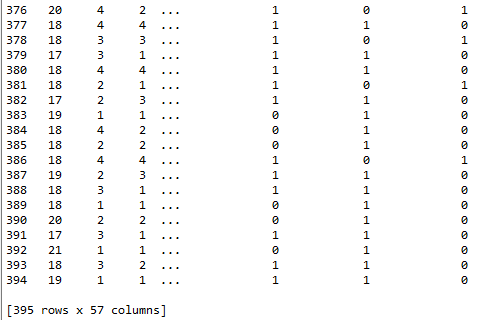
\includegraphics[width=5cm]{figures/1184003/chapter2/14.PNG}
		\caption{Hasil Soal 5.}
	\end{figure}
\item Soal 6
	\hfill\break
	\lstinputlisting[firstline=70, lastline=80]{src/1184003/chapter2/1184003.py}
	Graphviz adalah perangkat lunak visualisasi grafik open source. Visualisasi grafik adalah cara mewakili informasi struktural sebagai diagram grafik dan jaringan abstrak. 
	\item Soal 7
	\hfill\break
	\lstinputlisting[firstline=81, lastline=84]{src/1184003/chapter2/1184003.py}
	Tree.export graphviz merupakan fungsi yang menghasilkan representasi Graphviz dari decision tree, yang kemudian ditulis ke outfile.Disini akan menyimpan classifiernya, akan meng ekspor file student performance jika salah akan mengembalikan nilai fail. 
	\item Soal 8
	\hfill\break
	\lstinputlisting[firstline=85, lastline=87]{src/1184003/chapter2/1184003.py}
	Score juga disebut prediksi, dan merupakan proses menghasilkan nilai berdasarkan model pembelajaran mesin yang terlatih, diberi beberapa data input baru. Nilai atau skor yang dibuat dapat mewakili prediksi nilai masa depan, tetapi mereka juga mungkin mewakili kategori atau hasil yang mungkin. Jadi disini asahan akan memprediksi nilai dari medan test att dan test pass .
\item Soal 9
	\hfill\break
	\lstinputlisting[firstline=88, lastline=95]{src/1184003/chapter2/1184003.py}
	Skrip ini akan mengevaluasi score dengan validasi silang. Dimana variabel scores berisikan crossvalscore yang merupakan fungsi pembantu pada estimator dan dataset. Kemudian akan menampilkan score rata rata dan kurang lebih dua standar deviasi yang mencakup 95 persen score. 
	\item Soal 10
	\hfill\break
	\lstinputlisting[firstline=96, lastline=104]{src/1184003/chapter2/1184003.py}
	Pada skrip ini menunjukkan seberapa dalam tree itu. Semakin dalam tree, semakin banyak perpecahan yang dimilikinya dan menangkap lebih banyak informasi tentang data. variabel asahan akan mendefinisikan tree nya yang kemudian variabel scores akan mengevaluasi score dengan validasi silang. 
	\begin{figure}[h]
	\centering
		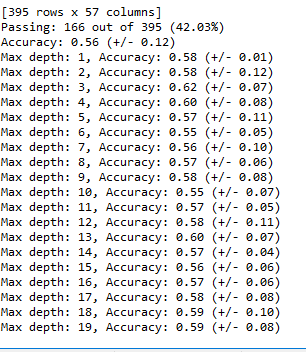
\includegraphics[width=2cm]{figures/1184003/chapter2/15.PNG}
		\caption{Hasil Soal 10.}
	\end{figure}
\item Soal 11
	\hfill\break
	\lstinputlisting[firstline=105, lastline=125]{src/1184003/chapter2/1184003.py}
	Depth acc akan membuat array kosong dengan mengembalikan array baru dengan bentuk dan tipe yang diberikan, tanpa menginisialisasi entri. Dengan 19 sebagai bentuk array kosong, 3 sebagai output data-type dan float urutan kolomutama (gaya Fortran) dalam memori. variabel asahan yang akan melakukan split score akan mengvalidasi score secara silang. 
	\item Soal 12
	\hfill\break
	\lstinputlisting[firstline=126, lastline=134]{src/1184003/chapter2/1184003.py}
	Mengimpor librari dari matplotlib yaitu pylot sebagai plt fig dan ax menggunakan subplots untuk membuat gambar dan satu set subplot. axerrorbar akan membuat error bar kemudian grafik akan ditampilkan menggunakan show.
	\begin{figure}
	\centering
		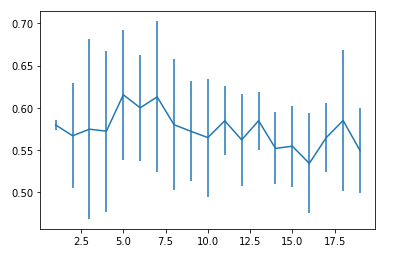
\includegraphics[width=10cm]{figures/1184003/chapter2/16.PNG}
		\caption{Hasil Soal 12.}
	\end{figure}
\end{enumerate}
\newpage\subsection{Penanganan Error}
\begin{enumerate}
	\item ScreenShoot Error
	\begin{figure}[h]
		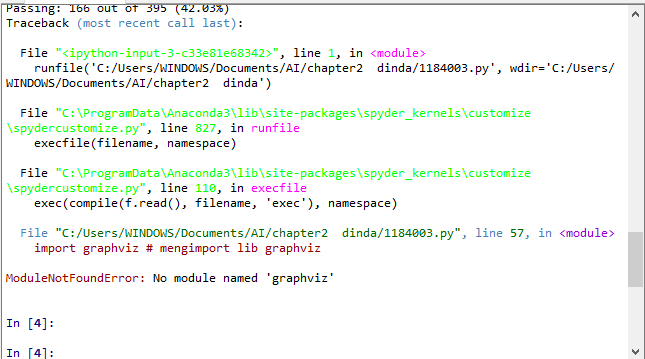
\includegraphics[width=10cm]{figures/1184003/chapter2/error1.png}
		\centering
		\caption{ModuleNotFoundError}
	\end{figure}
	\item Tuliskan Kode Error dan Jenis Error
	\begin{itemize}
	\lstinputlisting[firstline=70, lastline=80]{src/1184003/chapter2/1184003.py}
		\item ModuleNotFoundError
	\end{itemize}
	\item Cara Penangan Error
	\begin{itemize}
		\item ModuleNotFoundError
		\hfill\break
		Error terdapat pada kesalahan modul graphviz yang belum di install, solusinya ialah menginstall library tersebut di anaconda.
		\begin{figure}[h]
		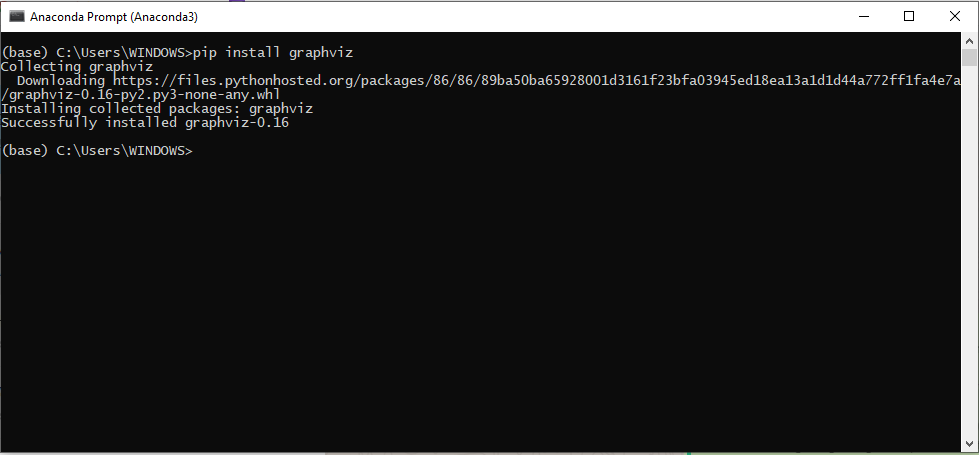
\includegraphics[width=10cm]{figures/1184003/chapter2/17.png}
		\centering
		\caption{ModuleNotFoundError}
	\end{figure}
	\end{itemize}
\end{enumerate}
	\subsection{Bukti Tidak Plagiat}
\begin{figure}[h]
	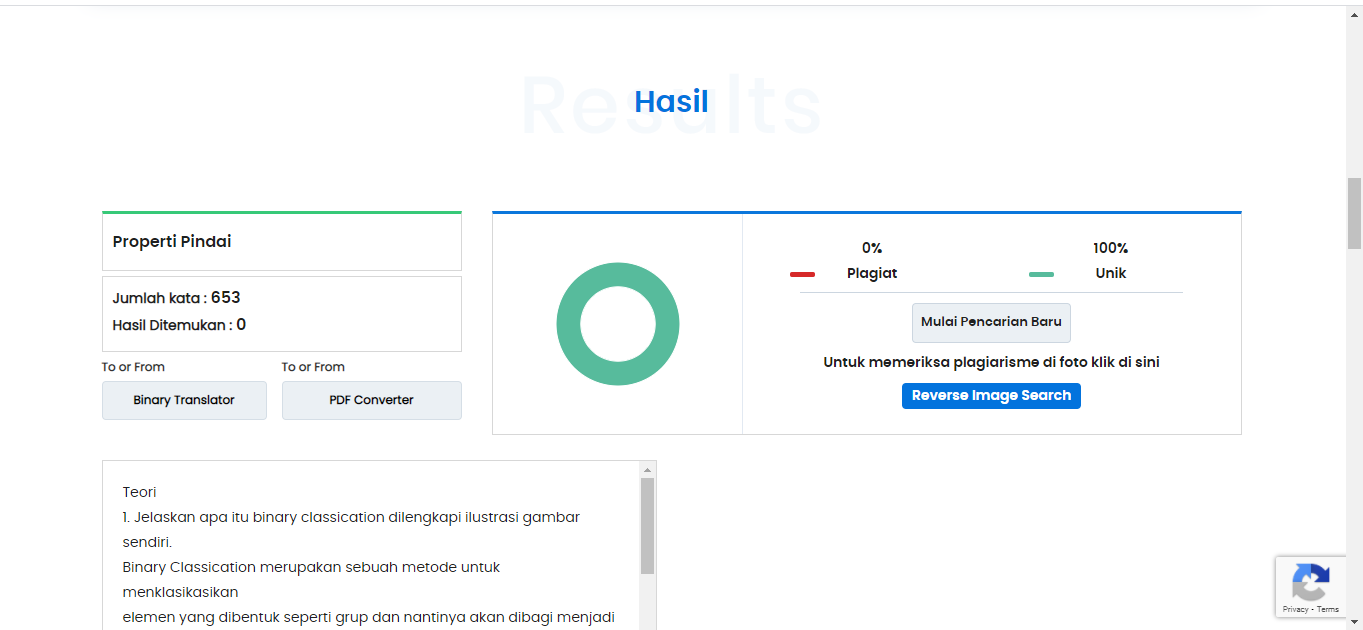
\includegraphics[width=10cm]{figures/1184003/chapter2/plagiat.png}
	\centering
	\caption{Bukti Tidak Melakukan Plagiat Chapter 2}
\end{figure}